% !TEX root=./adl.tex

% -----------------------------------------------------------------------
\begin{frame}{Why Parallelism?}

  Modern LLMs far exceed the memory of a single GPU.

  \vspace{0.5em}
  \begin{columns}
    \begin{column}{0.48\textwidth}
      \textbf{The scaling reality}
      \begin{itemize}
        \item GPT-3: 175B parameters
        \item Llama-3 405B: 405B parameters
        \item DeepSeek-V3: 671B parameters (MoE)
        \item Training requires storing weights, gradients, optimizer states, and activations
      \end{itemize}

      \vspace{0.5em}
      \textbf{Single GPU is not enough}
      \begin{itemize}
        \item H100 has 80\,GB HBM
        \item A 7B model in BF16 training already needs $\sim$112\,GB
        \item A 70B model needs $\sim$1120\,GB
      \end{itemize}
    \end{column}
    \begin{column}{0.48\textwidth}
      \textbf{Three fundamental challenges}~\cite{tazi2025ultrascale}
      \begin{enumerate}
        \item \emphdef{Memory}: Hard limit: if model state doesn't fit, training cannot begin
        \item \emphdef{Compute efficiency}: Minimize GPU idle time, maximize FLOP utilization (MFU)
        \item \emphdef{Communication overhead}: Minimize data transfer between GPUs, overlap with computation
      \end{enumerate}

      \vspace{0.5em}
      \begin{alertblock}{Goal}
        Distribute work across many GPUs such that training is both \emph{feasible} and \emph{efficient}.
      \end{alertblock}
    \end{column}
  \end{columns}
\end{frame}

% -----------------------------------------------------------------------
\begin{frame}{References}

  \begin{itemize}
    \item Material based on the Ultra-Scale Playbook~\cite{tazi2025ultrascale}
    \item Tensor \& pipeline parallelism at scale (Megatron-LM)~\cite{shoeybi2020megatronlm}
    \item Memory-efficient data parallelism via sharding (ZeRO)~\cite{rajbhandari2020zero}
    \item Pipeline parallelism with micro-batching (GPipe)~\cite{huang2019gpipe}
    \item Interleaved pipeline schedules, 3D parallelism~\cite{narayanan2021efficient}
    \item Selective activation recomputation~\cite{korthikanti2023selective}
    \item Mixed-precision training~\cite{micikevicius2018mixed}
    \item FlashAttention~\cite{dao2022flashattention}
    \item 4D parallelism at scale (Llama~3)~\cite{grattafiori2024llama3}
    \item FP8, DualPipe, expert parallelism (DeepSeek-V3)~\cite{deepseekai2024deepseekv3}
    \item Pathways system (PaLM)~\cite{chowdhery2023palm}
    \item 10k+ GPU training (MegaScale)~\cite{jiang2024megascale}
    \item PyTorch Distributed (FSDP)~\cite{li2020pytorch}
  \end{itemize}
\end{frame}

% -----------------------------------------------------------------------
\begin{frame}{Memory Breakdown: What Needs to Fit on a GPU?}

  Training a Transformer with $\Psi$ parameters in \emphdef{mixed precision} (BF16 compute + FP32 Adam):

  \vspace{0.3em}
  \begin{columns}
    \begin{column}{0.55\textwidth}
      \begin{itemize}
        \item \textbf{Weights} (BF16, $2\Psi$ bytes): Parameters used in forward/backward pass
        \item \textbf{Gradients} (BF16, $2\Psi$ bytes): One gradient per parameter, computed in backward pass
        \item \textbf{Master weights} (FP32, $4\Psi$ bytes): Full-precision copy of weights. Needed because weight updates $\theta \leftarrow \theta - \eta \cdot \Delta$ can be too small for BF16's limited mantissa (8-bit exponent, 7-bit mantissa)
        \item \textbf{1st moment} (FP32, $4\Psi$ bytes): Adam's running mean of gradients $m_t = \beta_1 m_{t-1} + (1-\beta_1) g_t$
        \item \textbf{2nd moment} (FP32, $4\Psi$ bytes): Adam's running mean of squared gradients $v_t = \beta_2 v_{t-1} + (1-\beta_2) g_t^2$
        \item \textbf{Activations}: Intermediate values saved for backward pass; depends on batch size, sequence length, number of layers
      \end{itemize}

      \vspace{0.3em}
      Total (excl.\ activations): $\mathbf{16\Psi}$ bytes per parameter
    \end{column}
    \begin{column}{0.42\textwidth}
      \begin{tikzpicture}[
        bar/.style={draw, minimum height=0.5cm, anchor=west, font=\scriptsize},
      ]
        % Fixed-size model state bars (anchor all at x=0)
        \node[bar, fill=blue!30,   minimum width=1.0cm] (w)  at (0, 3.2) {};
        \node[bar, fill=blue!18,   minimum width=1.0cm] (g)  at (0, 2.6) {};
        \node[bar, fill=orange!35, minimum width=2.0cm] (mc) at (0, 2.0) {};
        \node[bar, fill=orange!25, minimum width=2.0cm] (m1) at (0, 1.4) {};
        \node[bar, fill=orange!15, minimum width=2.0cm] (m2) at (0, 0.8) {};

        % Labels to the right
        \node[font=\scriptsize, anchor=west] at (w.east)  {~Weights \textbf{$2\Psi$}};
        \node[font=\scriptsize, anchor=west] at (g.east)  {~Gradients \textbf{$2\Psi$}};
        \node[font=\scriptsize, anchor=west] at (mc.east) {~FP32 master wt.\ \textbf{$4\Psi$}};
        \node[font=\scriptsize, anchor=west] at (m1.east) {~1st moment \textbf{$4\Psi$}};
        \node[font=\scriptsize, anchor=west] at (m2.east) {~2nd moment \textbf{$4\Psi$}};

        % Brace on the LEFT spanning all model-state bars
        \draw[decorate, decoration={brace, amplitude=5pt, mirror, raise=3pt}]
          (w.north west) -- (m2.south west)
          node[midway, left=10pt, font=\small, align=center] {$16\Psi$ \\ \scriptsize bytes};

        % Activations: variable-size bar with dashed right edge
        \node[bar, fill=red!15, minimum width=2.6cm, minimum height=0.5cm] (a) at (0, -0.1) {};
        % Dashed extension to show variable size
        \node[draw, dashed, fill=red!8, minimum width=1.0cm, minimum height=0.5cm, anchor=west] (aext) at (a.east) {};
        \node[font=\scriptsize, anchor=west] at (aext.east) {~Activations};
        \node[font=\tiny, gray, anchor=north] at ($(a.south)!0.5!(aext.south)$) {depends on $b$, $s$, $L$};
      \end{tikzpicture}
    \end{column}
  \end{columns}
\end{frame}

% -----------------------------------------------------------------------
\begin{frame}{Concrete Memory Requirements}

  \begin{center}
  \begin{tabular}{l r r r r}
    \toprule
    & \textbf{1B} & \textbf{7B} & \textbf{70B} & \textbf{405B} \\
    \midrule
    Weights (BF16)        & 2\,GB  & 14\,GB  & 140\,GB  & 810\,GB \\
    + Gradients (BF16)    & 4\,GB  & 28\,GB  & 280\,GB  & 1620\,GB \\
    + Optimizer (FP32)    & 16\,GB & 112\,GB & 1120\,GB & 6480\,GB \\
    + Activations$^*$     & ${\sim}$2\,GB & ${\sim}$8\,GB & ${\sim}$50\,GB & ${\sim}$200\,GB \\
    \midrule
    H100 GPUs needed      & 1      & 2       & 15       & 84 \\
    \bottomrule
  \end{tabular}
  \end{center}

  \vspace{0.5em}
  {\small Assuming 80\,GB per H100, mixed-precision training with Adam.
  $^*$Activations for mbs${}=1$, $s=4096$ with gradient checkpointing (see Section~\ref{sec:memory_tricks}); scales with batch size and sequence length.}

  \vspace{0.8em}
  \textbf{Key takeaway:}
  \begin{itemize}
    \item Even a 7B model doesn't fit on a single GPU for training
    \item We need strategies to \emph{distribute} model state across GPUs
    \item This is where the \emph{five dimensions} of parallelism come in
  \end{itemize}
\end{frame}

% -----------------------------------------------------------------------
\begin{frame}{Overview of Parallelism Strategies}

  Five complementary dimensions, each splitting along a different axis:

  \vspace{0.3em}
  \begin{center}
  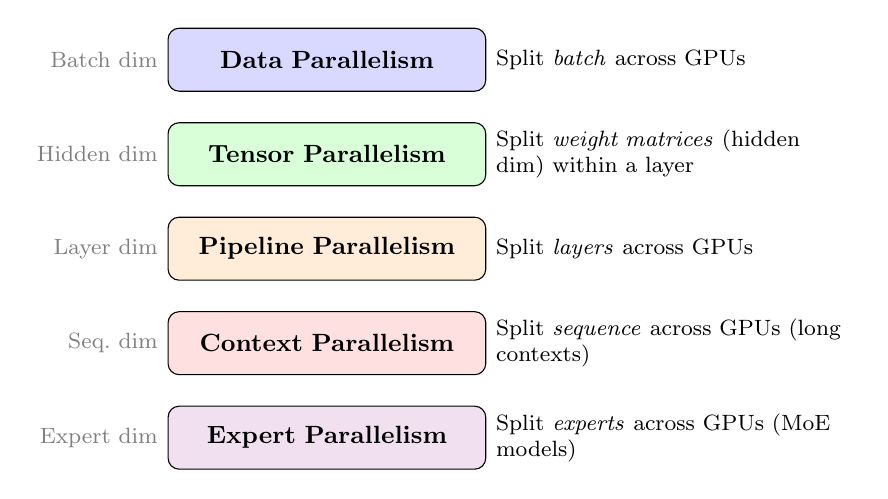
\begin{tikzpicture}[
    strat/.style={draw, rounded corners, text width=3.8cm, align=center, font=\small, minimum height=0.8cm},
    lbl/.style={font=\footnotesize, text width=4.5cm, align=left},
  ]
    \node[strat, fill=blue!15]   (dp)  at (0, 2.0) {\textbf{Data Parallelism}};
    \node[strat, fill=green!15]  (tp)  at (0, 0.8) {\textbf{Tensor Parallelism}};
    \node[strat, fill=orange!15] (pp)  at (0,-0.4) {\textbf{Pipeline Parallelism}};
    \node[strat, fill=red!12]    (cp)  at (0,-1.6) {\textbf{Context Parallelism}};
    \node[strat, fill=violet!12] (ep)  at (0,-2.8) {\textbf{Expert Parallelism}};

    \node[lbl, anchor=west] at (dp.east)  {Split \emph{batch} across GPUs};
    \node[lbl, anchor=west] at (tp.east)  {Split \emph{weight matrices} (hidden dim) within a layer};
    \node[lbl, anchor=west] at (pp.east)  {Split \emph{layers} across GPUs};
    \node[lbl, anchor=west] at (cp.east)  {Split \emph{sequence} across GPUs (long contexts)};
    \node[lbl, anchor=west] at (ep.east)  {Split \emph{experts} across GPUs (MoE models)};

    \node[font=\footnotesize, gray, anchor=east] at (dp.west)  {Batch dim};
    \node[font=\footnotesize, gray, anchor=east] at (tp.west)  {Hidden dim};
    \node[font=\footnotesize, gray, anchor=east] at (pp.west)  {Layer dim};
    \node[font=\footnotesize, gray, anchor=east] at (cp.west)  {Seq.\ dim};
    \node[font=\footnotesize, gray, anchor=east] at (ep.west)  {Expert dim};
  \end{tikzpicture}
  \end{center}

  \vspace{0.3em}
  \begin{alertblock}{5D Parallelism}
    State-of-the-art training (Llama-3, DeepSeek-V3) combines \emph{all five} dimensions simultaneously.
    The global batch size becomes: $\text{GBS} = \text{mbs} \times \text{grad\_acc} \times \text{DP}$.
  \end{alertblock}
\end{frame}

% -----------------------------------------------------------------------
\begin{frame}{GPU Interconnects and Topology}

  Communication speed between GPUs critically determines which parallelism strategies are practical.

  \vspace{0.5em}
  \begin{columns}
    \begin{column}{0.55\textwidth}
      \textbf{Intra-node (within a server):}
      \begin{itemize}
        \item \emphdef{NVLink / NVSwitch}: Up to 900\,GB/s (H100)
        \item 8 GPUs fully connected within one node
        \item Used for \emph{Tensor Parallelism} (frequent, latency-sensitive communication)
      \end{itemize}

      \vspace{0.5em}
      \textbf{Inter-node (across servers):}
      \begin{itemize}
        \item \emphdef{InfiniBand / RoCE}: $\sim$50--400\,Gb/s per link
        \item Much slower than NVLink ($\sim$5--20$\times$)
        \item Used for \emph{Data \& Pipeline Parallelism} (less frequent, larger messages)
      \end{itemize}
    \end{column}
    \begin{column}{0.42\textwidth}
      \begin{tikzpicture}[
        gpu/.style={draw, rounded corners=1.5pt, fill=slide_green!60,
          minimum width=0.4cm, minimum height=0.7cm, font=\tiny, inner sep=0.5pt},
        nvsw/.style={draw, rounded corners=1.5pt, fill=orange!25,
          minimum width=3.5cm, minimum height=0.18cm, font=\tiny, inner sep=1pt},
        nodebox/.style={draw, rounded corners=3pt, inner sep=3pt, fill=blue!4},
        ibnet/.style={draw, rounded corners=2pt, fill=red!12,
          minimum width=3.8cm, minimum height=0.22cm, font=\tiny, inner sep=1pt},
      ]
        \def\gs{0.44}   % GPU horizontal spacing
        \def\cx{1.54}   % center x = 7*\gs/2

        % ========= Node 0 =========
        \foreach \i in {0,...,7} {
          \node[gpu] (a\i) at (\i*\gs, 0) {G\i};
        }
        \node[nvsw] (nv0) at (\cx, -0.58) {NVSwitch};
        \begin{scope}[on background layer]
          \node[nodebox, fit=(a0)(a7)(nv0),
                label={[font=\tiny\bfseries]above:Node 0}] (n0) {};
        \end{scope}
        % NVLink: GPUs <-> NVSwitch
        \foreach \i in {0,...,7} {
          \draw[blue!60, line width=0.7pt] (a\i.south) -- (a\i.south |- nv0.north);
        }

        % ========= Node 1 =========
        \foreach \i in {0,...,7} {
          \node[gpu] (b\i) at (\i*\gs, -2.2) {G\i};
        }
        \node[nvsw] (nv1) at (\cx, -2.78) {NVSwitch};
        \begin{scope}[on background layer]
          \node[nodebox, fit=(b0)(b7)(nv1),
                label={[font=\tiny\bfseries]below:Node 1}] (n1) {};
        \end{scope}
        \foreach \i in {0,...,7} {
          \draw[blue!60, line width=0.7pt] (b\i.south) -- (b\i.south |- nv1.north);
        }

        % ========= InfiniBand Network =========
        \node[ibnet] (ib) at ($(n0.south)!0.5!(n1.north)$) {InfiniBand};
        % Parallel links: Node 0 <-> IB <-> Node 1
        \foreach \i in {0,3,4,7} {
          \draw[red!70, line width=0.6pt, densely dashed]
            (a\i |- n0.south) -- (a\i |- ib.north);
          \draw[red!70, line width=0.6pt, densely dashed]
            (b\i |- ib.south) -- (b\i |- n1.north);
        }

        % ========= Legend =========
        \node[anchor=north west, font=\tiny] (leg1) at (-0.1, -3.7) {%
          \textcolor{blue!60}{\rule{0.4cm}{1.5pt}}~NVLink (900\,GB/s)};
        \node[anchor=north west, font=\tiny] at (leg1.south west) {%
          \textcolor{red!70}{\rule[0.4ex]{0.12cm}{0.8pt}}%
          \kern0.5pt\textcolor{red!70}{\rule[0.4ex]{0.12cm}{0.8pt}}%
          \kern0.5pt\textcolor{red!70}{\rule[0.4ex]{0.08cm}{0.8pt}}~%
          IB (50--400\,Gb/s)};
      \end{tikzpicture}
    \end{column}
  \end{columns}

  \vspace{0.3em}
  \textbf{Rule of thumb:} Use TP within a node (degree $\leq 8$), DP and PP across nodes.
\end{frame}

% -----------------------------------------------------------------------
\begin{frame}{Collective Communication Operations}

  Parallelism strategies rely on a small set of \emphdef{collective operations}:

  \vspace{0.3em}
  \begin{center}
  \begin{tabular}{l p{7.5cm}}
    \toprule
    \textbf{Operation} & \textbf{Description} \\
    \midrule
    \textbf{Broadcast}       & One GPU sends data to all others \\
    \textbf{Reduce}          & Combine (e.g.\ sum) data from all GPUs to one \\
    \textbf{AllReduce}       & Reduce + broadcast result to all GPUs \\
    \textbf{Scatter}         & Split data from one GPU, send chunks to each \\
    \textbf{Gather}          & Collect chunks from all GPUs to one \\
    \textbf{AllGather}       & Gather + broadcast: every GPU gets the full result \\
    \textbf{ReduceScatter}   & Reduce + scatter: each GPU gets a reduced chunk \\
    \textbf{AllToAll}        & Each GPU sends a different chunk to each other GPU \\
    \bottomrule
  \end{tabular}
  \end{center}

  \vspace{0.3em}
  \begin{itemize}
    \item Implemented in \textbf{NCCL} (NVIDIA Collective Communications Library)
    \item \emphdef{AllReduce} is the workhorse of data parallelism (gradient sync)
    \item \emphdef{AllGather} + \emphdef{ReduceScatter} are key for ZeRO / FSDP
  \end{itemize}
\end{frame}

% -----------------------------------------------------------------------
\begin{frame}{Broadcast}

  \textbf{One GPU sends the same data to all other GPUs.}

  \vspace{0.3em}
  \begin{columns}
    \begin{column}{0.55\textwidth}
      \begin{center}
      \begin{tikzpicture}[
        gpu/.style={draw, rounded corners=2pt, minimum width=1.2cm,
          minimum height=0.7cm, font=\small, inner sep=2pt},
        data/.style={font=\scriptsize},
        arrow/.style={->, thick, blue!60!black, line width=0.9pt,
          shorten >=1pt, shorten <=1pt},
      ]
        % Before
        \node[font=\small\bfseries] at (0, 2.8) {Before};
        \node[gpu, fill=gray!12]  (b0) at (0, 2.0) {GPU 0};
        \node[gpu, fill=gray!12]  (b1) at (0, 1.1) {GPU 1};
        \node[gpu, fill=blue!25]  (b2) at (0, 0.2) {GPU 2};
        \node[gpu, fill=gray!12]  (b3) at (0,-0.7) {GPU 3};

        \node[data, anchor=west, gray]          at (b0.east) {~$[\,]$};
        \node[data, anchor=west, gray]          at (b1.east) {~$[\,]$};
        \node[data, anchor=west, blue!70!black] at (b2.east) {~$[A]$};
        \node[data, anchor=west, gray]          at (b3.east) {~$[\,]$};

        % After
        \node[font=\small\bfseries] at (4.6, 2.8) {After};
        \node[gpu, fill=blue!15]  (a0) at (4.6, 2.0) {GPU 0};
        \node[gpu, fill=blue!15]  (a1) at (4.6, 1.1) {GPU 1};
        \node[gpu, fill=blue!25]  (a2) at (4.6, 0.2) {GPU 2};
        \node[gpu, fill=blue!15]  (a3) at (4.6,-0.7) {GPU 3};

        \node[data, anchor=west, blue!70!black] at (a0.east) {~$[A]$};
        \node[data, anchor=west, blue!70!black] at (a1.east) {~$[A]$};
        \node[data, anchor=west, blue!70!black] at (a2.east) {~$[A]$};
        \node[data, anchor=west, blue!70!black] at (a3.east) {~$[A]$};

        % Arrows from b2 to each GPU; first 10% transparent to avoid [A] overlap
        \foreach \tgt in {a0,a1,a3} {
          \coordinate (mid) at ($(b2.east)!0.15!(\tgt.west)$);
          \draw[draw=none] (b2.east) -- (mid);
          \draw[arrow] (mid) -- (\tgt.west);
        }
      \end{tikzpicture}
      \end{center}
    \end{column}
    \begin{column}{0.42\textwidth}
      \begin{itemize}
        \item \textbf{Root} GPU holds the data, all others receive a copy
        \item Data volume transferred: $(N{-}1) \cdot |A|$ in the naive case; tree-based broadcast reduces latency to $O(\log N)$ steps
        \item \textbf{Use cases:}
          \begin{itemize}
            \item Distributing initial model weights to all GPUs at startup
            \item Sharing hyperparameters or random seeds
          \end{itemize}
      \end{itemize}
    \end{column}
  \end{columns}
\end{frame}

% -----------------------------------------------------------------------
\begin{frame}{Naive vs.\ Tree-Based Broadcast}

  \begin{columns}
    \begin{column}{0.48\textwidth}
      \centering
      \textbf{Naive:} $N{-}1$ sequential steps

      \vspace{0.4em}
      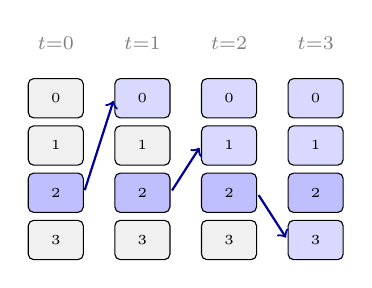
\begin{tikzpicture}[
        gpu/.style={draw, rounded corners=2pt, minimum width=0.7cm,
          minimum height=0.5cm, font=\tiny, inner sep=1pt},
        arr/.style={->, thick, blue!60!black, line width=0.8pt,
          shorten >=1pt, shorten <=1pt},
        steplbl/.style={font=\scriptsize\bfseries, gray},
      ]
        \def\sx{1.1}  % horizontal step spacing

        % Step 0
        \node[steplbl] at (0, 1.8) {$t{=}0$};
        \node[gpu, fill=gray!12]  (s0g0) at (0, 1.1) {0};
        \node[gpu, fill=gray!12]  (s0g1) at (0, 0.5) {1};
        \node[gpu, fill=blue!25]  (s0g2) at (0,-0.1) {2};
        \node[gpu, fill=gray!12]  (s0g3) at (0,-0.7) {3};

        % Step 1: GPU 2 -> GPU 0
        \node[steplbl] at (\sx, 1.8) {$t{=}1$};
        \node[gpu, fill=blue!15]  (s1g0) at (\sx, 1.1) {0};
        \node[gpu, fill=gray!12]  (s1g1) at (\sx, 0.5) {1};
        \node[gpu, fill=blue!25]  (s1g2) at (\sx,-0.1) {2};
        \node[gpu, fill=gray!12]  (s1g3) at (\sx,-0.7) {3};
        \draw[arr] (s0g2.east) -- (s1g0.west);

        % Step 2: GPU 2 -> GPU 1
        \node[steplbl] at (2*\sx, 1.8) {$t{=}2$};
        \node[gpu, fill=blue!15]  (s2g0) at (2*\sx, 1.1) {0};
        \node[gpu, fill=blue!15]  (s2g1) at (2*\sx, 0.5) {1};
        \node[gpu, fill=blue!25]  (s2g2) at (2*\sx,-0.1) {2};
        \node[gpu, fill=gray!12]  (s2g3) at (2*\sx,-0.7) {3};
        \draw[arr] (s1g2.east) -- (s2g1.west);

        % Step 3: GPU 2 -> GPU 3
        \node[steplbl] at (3*\sx, 1.8) {$t{=}3$};
        \node[gpu, fill=blue!15]  (s3g0) at (3*\sx, 1.1) {0};
        \node[gpu, fill=blue!15]  (s3g1) at (3*\sx, 0.5) {1};
        \node[gpu, fill=blue!25]  (s3g2) at (3*\sx,-0.1) {2};
        \node[gpu, fill=blue!15]  (s3g3) at (3*\sx,-0.7) {3};
        \draw[arr] (s2g2.east) -- (s3g3.west);
      \end{tikzpicture}
    \end{column}
    \begin{column}{0.48\textwidth}
      \centering
      \textbf{Tree-based:} $\lceil \log_2 N \rceil$ steps

      \vspace{0.4em}
      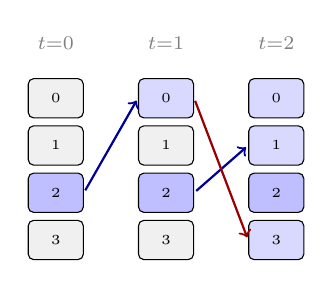
\begin{tikzpicture}[
        gpu/.style={draw, rounded corners=2pt, minimum width=0.7cm,
          minimum height=0.5cm, font=\tiny, inner sep=1pt},
        arr/.style={->, thick, blue!60!black, line width=0.8pt,
          shorten >=1pt, shorten <=1pt},
        steplbl/.style={font=\scriptsize\bfseries, gray},
      ]
        \def\sx{1.4}  % horizontal step spacing

        % Step 0
        \node[steplbl] at (0, 1.8) {$t{=}0$};
        \node[gpu, fill=gray!12]  (s0g0) at (0, 1.1) {0};
        \node[gpu, fill=gray!12]  (s0g1) at (0, 0.5) {1};
        \node[gpu, fill=blue!25]  (s0g2) at (0,-0.1) {2};
        \node[gpu, fill=gray!12]  (s0g3) at (0,-0.7) {3};

        % Step 1: GPU 2 -> GPU 0
        \node[steplbl] at (\sx, 1.8) {$t{=}1$};
        \node[gpu, fill=blue!15]  (s1g0) at (\sx, 1.1) {0};
        \node[gpu, fill=gray!12]  (s1g1) at (\sx, 0.5) {1};
        \node[gpu, fill=blue!25]  (s1g2) at (\sx,-0.1) {2};
        \node[gpu, fill=gray!12]  (s1g3) at (\sx,-0.7) {3};
        \draw[arr] (s0g2.east) -- (s1g0.west);

        % Step 2: GPU 2 -> GPU 1  AND  GPU 0 -> GPU 3 (parallel!)
        \node[steplbl] at (2*\sx, 1.8) {$t{=}2$};
        \node[gpu, fill=blue!15]  (s2g0) at (2*\sx, 1.1) {0};
        \node[gpu, fill=blue!15]  (s2g1) at (2*\sx, 0.5) {1};
        \node[gpu, fill=blue!25]  (s2g2) at (2*\sx,-0.1) {2};
        \node[gpu, fill=blue!15]  (s2g3) at (2*\sx,-0.7) {3};
        \draw[arr] (s1g2.east) -- (s2g1.west);
        \draw[arr, red!60!black] (s1g0.east) -- (s2g3.west);
      \end{tikzpicture}
    \end{column}
  \end{columns}

  \vspace{0.6em}
  \begin{itemize}
    \item Tree-based: GPUs that already have the data \textbf{help forward} it
    \item At step $t{=}2$, GPU~2 and GPU~0 send \emph{in parallel} (red arrow = forwarded by receiver)
    \item With $N{=}1024$ GPUs: 10 steps instead of 1023
    \item NCCL uses ring and tree topologies under the hood
  \end{itemize}
\end{frame}

% -----------------------------------------------------------------------
\begin{frame}{Reduce}

  \textbf{Combine data from all GPUs onto one root GPU} (e.g.\ sum, max).

  \vspace{0.3em}
  \begin{columns}
    \begin{column}{0.55\textwidth}
      \begin{center}
      \begin{tikzpicture}[
        gpu/.style={draw, rounded corners=2pt, minimum width=1.2cm,
          minimum height=0.7cm, font=\small, inner sep=2pt},
        data/.style={font=\scriptsize},
        arrow/.style={->, thick, blue!60!black, line width=0.9pt,
          shorten >=1pt, shorten <=1pt},
      ]
        % Before
        \node[font=\small\bfseries] at (0, 2.8) {Before};
        \node[gpu, fill=red!15]    (b0) at (0, 2.0) {GPU 0};
        \node[gpu, fill=green!15]  (b1) at (0, 1.1) {GPU 1};
        \node[gpu, fill=orange!15] (b2) at (0, 0.2) {GPU 2};
        \node[gpu, fill=violet!15] (b3) at (0,-0.7) {GPU 3};

        \node[data, anchor=west, red!70!black]    at (b0.east) {~$[A]$};
        \node[data, anchor=west, green!50!black]  at (b1.east) {~$[B]$};
        \node[data, anchor=west, orange!70!black] at (b2.east) {~$[C]$};
        \node[data, anchor=west, violet!70!black] at (b3.east) {~$[D]$};

        % After
        \node[font=\small\bfseries] at (4.6, 2.8) {After};
        \node[gpu, fill=gray!12]  (a0) at (4.6, 2.0) {GPU 0};
        \node[gpu, fill=gray!12]  (a1) at (4.6, 1.1) {GPU 1};
        \node[gpu, fill=blue!25]  (a2) at (4.6, 0.2) {GPU 2};
        \node[gpu, fill=gray!12]  (a3) at (4.6,-0.7) {GPU 3};

        \node[data, anchor=west, gray]          at (a0.east) {~$[\,]$};
        \node[data, anchor=west, gray]          at (a1.east) {~$[\,]$};
        \node[data, anchor=west, blue!70!black] at (a2.east) {~$[A{+}B{+}C{+}D]$};
        \node[data, anchor=west, gray]          at (a3.east) {~$[\,]$};

        % Arrows from each GPU to root GPU 2; first 15% transparent
        \foreach \src in {b0,b1,b3} {
          \coordinate (mid) at ($(\src.east)!0.15!(a2.west)$);
          \draw[draw=none] (\src.east) -- (mid);
          \draw[arrow] (mid) -- (a2.west);
        }
      \end{tikzpicture}
      \end{center}
    \end{column}
    \begin{column}{0.42\textwidth}
      \begin{itemize}
        \item Each GPU holds local data; the \textbf{root} receives the combined result
        \item Reduction operator is typically \emph{sum}, but can be max, min, product, etc.
        \item Inverse of broadcast: many $\to$ one
        \item \textbf{Implementation:} Tree-based reduce (mirror of tree broadcast): partial sums flow up a binary tree in $O(\log N)$ steps
        \item \textbf{Use cases:}
          \begin{itemize}
            \item Summing partial loss values across GPUs
            \item Aggregating metrics (accuracy, counts)
          \end{itemize}
      \end{itemize}
    \end{column}
  \end{columns}
\end{frame}

% -----------------------------------------------------------------------
\begin{frame}{Scatter}

  \textbf{Split data from one GPU and distribute chunks to each GPU.}

  \vspace{0.3em}
  \begin{columns}
    \begin{column}{0.55\textwidth}
      \begin{center}
      \begin{tikzpicture}[
        gpu/.style={draw, rounded corners=2pt, minimum width=1.2cm,
          minimum height=0.7cm, font=\small, inner sep=2pt},
        data/.style={font=\scriptsize},
        arrow/.style={->, thick, blue!60!black, line width=0.9pt,
          shorten >=1pt, shorten <=1pt},
      ]
        % Before
        \node[font=\small\bfseries] at (0, 2.8) {Before};
        \node[gpu, fill=blue!25]  (b0) at (0, 2.0) {GPU 0};
        \node[gpu, fill=gray!12]  (b1) at (0, 1.1) {GPU 1};
        \node[gpu, fill=gray!12]  (b2) at (0, 0.2) {GPU 2};
        \node[gpu, fill=gray!12]  (b3) at (0,-0.7) {GPU 3};

        \node[data, anchor=west, blue!70!black] at (b0.east) {~$[A,B,C,D]$};
        \node[data, anchor=west, gray]          at (b1.east) {~$[\,]$};
        \node[data, anchor=west, gray]          at (b2.east) {~$[\,]$};
        \node[data, anchor=west, gray]          at (b3.east) {~$[\,]$};

        % After
        \node[font=\small\bfseries] at (4.6, 2.8) {After};
        \node[gpu, fill=red!15]    (a0) at (4.6, 2.0) {GPU 0};
        \node[gpu, fill=green!15]  (a1) at (4.6, 1.1) {GPU 1};
        \node[gpu, fill=orange!15] (a2) at (4.6, 0.2) {GPU 2};
        \node[gpu, fill=violet!15] (a3) at (4.6,-0.7) {GPU 3};

        \node[data, anchor=west, red!70!black]    at (a0.east) {~$[A]$};
        \node[data, anchor=west, green!50!black]  at (a1.east) {~$[B]$};
        \node[data, anchor=west, orange!70!black] at (a2.east) {~$[C]$};
        \node[data, anchor=west, violet!70!black] at (a3.east) {~$[D]$};

        % Arrows from GPU 0 to each; first 15% transparent
        \foreach \tgt in {a1,a2,a3} {
          \coordinate (mid) at ($(b0.east)!0.25!(\tgt.west)$);
          \draw[draw=none] (b0.east) -- (mid);
          \draw[arrow] (mid) -- (\tgt.west);
        }
      \end{tikzpicture}
      \end{center}
    \end{column}
    \begin{column}{0.42\textwidth}
      \begin{itemize}
        \item One GPU holds the \emph{full} data, which is split into $N$ equal chunks
        \item Each GPU receives exactly one chunk
        \item Inverse of gather: one $\to$ many (partitioned)
        \item Unlike broadcast, each GPU gets a \emph{different} piece
        \item \textbf{Implementation:} Direct point-to-point sends from root; can also use tree-based scatter in $O(\log N)$ steps
        \item \textbf{Use cases:}
          \begin{itemize}
            \item Distributing sharded optimizer states (ZeRO)
            \item Partitioning input batches
          \end{itemize}
      \end{itemize}
    \end{column}
  \end{columns}
\end{frame}

% -----------------------------------------------------------------------
\begin{frame}{Gather}

  \textbf{Collect chunks from all GPUs onto one root GPU.}

  \vspace{0.3em}
  \begin{columns}
    \begin{column}{0.55\textwidth}
      \begin{center}
      \begin{tikzpicture}[
        gpu/.style={draw, rounded corners=2pt, minimum width=1.2cm,
          minimum height=0.7cm, font=\small, inner sep=2pt},
        data/.style={font=\scriptsize},
        arrow/.style={->, thick, blue!60!black, line width=0.9pt,
          shorten >=1pt, shorten <=1pt},
      ]
        % Before
        \node[font=\small\bfseries] at (0, 2.8) {Before};
        \node[gpu, fill=red!15]    (b0) at (0, 2.0) {GPU 0};
        \node[gpu, fill=green!15]  (b1) at (0, 1.1) {GPU 1};
        \node[gpu, fill=orange!15] (b2) at (0, 0.2) {GPU 2};
        \node[gpu, fill=violet!15] (b3) at (0,-0.7) {GPU 3};

        \node[data, anchor=west, red!70!black]    at (b0.east) {~$[A]$};
        \node[data, anchor=west, green!50!black]  at (b1.east) {~$[B]$};
        \node[data, anchor=west, orange!70!black] at (b2.east) {~$[C]$};
        \node[data, anchor=west, violet!70!black] at (b3.east) {~$[D]$};

        % After
        \node[font=\small\bfseries] at (4.6, 2.8) {After};
        \node[gpu, fill=blue!25]  (a0) at (4.6, 2.0) {GPU 0};
        \node[gpu, fill=gray!12]  (a1) at (4.6, 1.1) {GPU 1};
        \node[gpu, fill=gray!12]  (a2) at (4.6, 0.2) {GPU 2};
        \node[gpu, fill=gray!12]  (a3) at (4.6,-0.7) {GPU 3};

        \node[data, anchor=west, blue!70!black] at (a0.east) {~$[A,B,C,D]$};
        \node[data, anchor=west, gray]          at (a1.east) {~$[\,]$};
        \node[data, anchor=west, gray]          at (a2.east) {~$[\,]$};
        \node[data, anchor=west, gray]          at (a3.east) {~$[\,]$};

        % Arrows from each GPU to root GPU 0; first 15% transparent
        \foreach \src in {b1,b2,b3} {
          \coordinate (mid) at ($(\src.east)!0.15!(a0.west)$);
          \draw[draw=none] (\src.east) -- (mid);
          \draw[arrow] (mid) -- (a0.west);
        }
      \end{tikzpicture}
      \end{center}
    \end{column}
    \begin{column}{0.42\textwidth}
      \begin{itemize}
        \item Each GPU holds one chunk; the \textbf{root} collects and concatenates all chunks
        \item Inverse of scatter: many $\to$ one (concatenated)
        \item Unlike reduce, chunks are \emph{concatenated}, not combined with an operator
        \item \textbf{Implementation:} Direct point-to-point sends to root; mirror of scatter
        \item \textbf{Use cases:}
          \begin{itemize}
            \item Collecting partial results (e.g.\ activations from pipeline stages)
            \item Reassembling sharded tensors on one GPU for checkpointing
          \end{itemize}
      \end{itemize}
    \end{column}
  \end{columns}
\end{frame}

% -----------------------------------------------------------------------
\begin{frame}{AllReduce}

  \textbf{Reduce data across all GPUs, then distribute the result to every GPU.}
  Equivalent to Reduce + Broadcast, but implemented more efficiently.

  \vspace{0.3em}
  \begin{columns}
    \begin{column}{0.55\textwidth}
      \begin{center}
      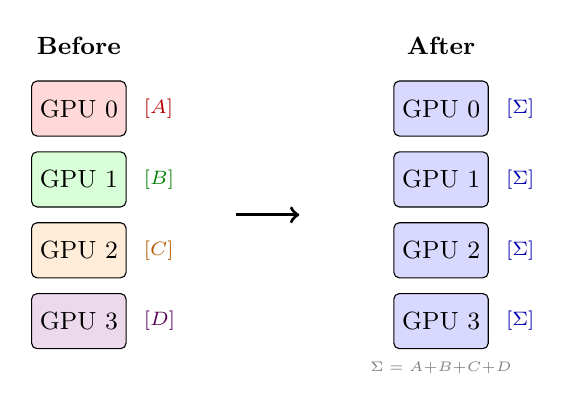
\begin{tikzpicture}[
        gpu/.style={draw, rounded corners=2pt, minimum width=1.2cm,
          minimum height=0.7cm, font=\small, inner sep=2pt},
        data/.style={font=\scriptsize},
      ]
        % Before
        \node[font=\small\bfseries] at (0, 2.8) {Before};
        \node[gpu, fill=red!15]    (b0) at (0, 2.0) {GPU 0};
        \node[gpu, fill=green!15]  (b1) at (0, 1.1) {GPU 1};
        \node[gpu, fill=orange!15] (b2) at (0, 0.2) {GPU 2};
        \node[gpu, fill=violet!15] (b3) at (0,-0.7) {GPU 3};

        \node[data, anchor=west, red!70!black]    at (b0.east) {~$[A]$};
        \node[data, anchor=west, green!50!black]  at (b1.east) {~$[B]$};
        \node[data, anchor=west, orange!70!black] at (b2.east) {~$[C]$};
        \node[data, anchor=west, violet!70!black] at (b3.east) {~$[D]$};

        % Arrow
        \draw[->, thick, line width=1.2pt] (2.0, 0.65) -- (2.8, 0.65);

        % After
        \node[font=\small\bfseries] at (4.6, 2.8) {After};
        \node[gpu, fill=blue!15]  (a0) at (4.6, 2.0) {GPU 0};
        \node[gpu, fill=blue!15]  (a1) at (4.6, 1.1) {GPU 1};
        \node[gpu, fill=blue!15]  (a2) at (4.6, 0.2) {GPU 2};
        \node[gpu, fill=blue!15]  (a3) at (4.6,-0.7) {GPU 3};

        \node[data, anchor=west, blue!70!black] at (a0.east) {~$[\Sigma]$};
        \node[data, anchor=west, blue!70!black] at (a1.east) {~$[\Sigma]$};
        \node[data, anchor=west, blue!70!black] at (a2.east) {~$[\Sigma]$};
        \node[data, anchor=west, blue!70!black] at (a3.east) {~$[\Sigma]$};

        \node[font=\tiny, gray] at (4.6, -1.3) {$\Sigma = A{+}B{+}C{+}D$};
      \end{tikzpicture}
      \end{center}
    \end{column}
    \begin{column}{0.42\textwidth}
      \begin{itemize}
        \item Every GPU starts with local data and ends with the \emph{same} reduced result
        \item \textbf{The} workhorse of data parallelism: synchronize gradients across all replicas
        \item \textbf{Implementation:} Ring AllReduce (see next slide), bandwidth-optimal
        \item \textbf{Use cases:}
          \begin{itemize}
            \item Gradient synchronization in data parallelism
            \item Averaging batch statistics (e.g.\ BatchNorm)
          \end{itemize}
      \end{itemize}
    \end{column}
  \end{columns}
\end{frame}

% -----------------------------------------------------------------------
\begin{frame}{Ring AllReduce}

  \textbf{Bandwidth-optimal} AllReduce: GPUs arranged in a logical ring, two phases.

  \vspace{0.2em}
  \begin{columns}
    \begin{column}{0.48\textwidth}
      \centering
      \textbf{Phase 1: ReduceScatter}

      \vspace{0.3em}
      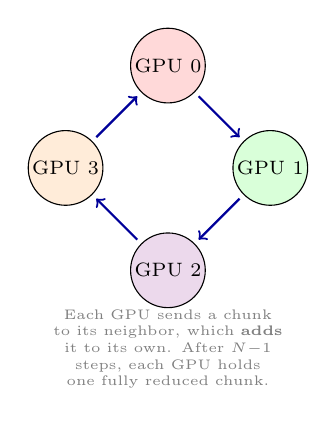
\begin{tikzpicture}[
        gpu/.style={draw, circle, minimum size=0.9cm, font=\scriptsize, inner sep=1pt},
        arr/.style={->, thick, blue!60!black, line width=0.8pt, shorten >=2pt, shorten <=2pt},
      ]
        \node[gpu, fill=red!15]    (g0) at (90:1.3)  {GPU 0};
        \node[gpu, fill=green!15]  (g1) at (0:1.3)   {GPU 1};
        \node[gpu, fill=violet!15] (g2) at (270:1.3) {GPU 2};
        \node[gpu, fill=orange!15] (g3) at (180:1.3) {GPU 3};

        % Ring arrows
        \draw[arr] (g0) -- (g1);
        \draw[arr] (g1) -- (g2);
        \draw[arr] (g2) -- (g3);
        \draw[arr] (g3) -- (g0);

        % Label
        \node[font=\tiny, gray, text width=3cm, align=center] at (0, -2.3)
          {Each GPU sends a chunk to its neighbor, which \textbf{adds} it to its own.
           After $N{-}1$ steps, each GPU holds one fully reduced chunk.};
      \end{tikzpicture}
    \end{column}
    \begin{column}{0.48\textwidth}
      \centering
      \textbf{Phase 2: AllGather}

      \vspace{0.3em}
      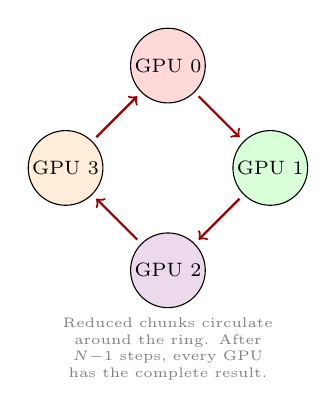
\begin{tikzpicture}[
        gpu/.style={draw, circle, minimum size=0.9cm, font=\scriptsize, inner sep=1pt},
        arr/.style={->, thick, red!60!black, line width=0.8pt, shorten >=2pt, shorten <=2pt},
      ]
        \node[gpu, fill=red!15]    (g0) at (90:1.3)  {GPU 0};
        \node[gpu, fill=green!15]  (g1) at (0:1.3)   {GPU 1};
        \node[gpu, fill=violet!15] (g2) at (270:1.3) {GPU 2};
        \node[gpu, fill=orange!15] (g3) at (180:1.3) {GPU 3};

        % Ring arrows
        \draw[arr] (g0) -- (g1);
        \draw[arr] (g1) -- (g2);
        \draw[arr] (g2) -- (g3);
        \draw[arr] (g3) -- (g0);

        % Label
        \node[font=\tiny, gray, text width=3cm, align=center] at (0, -2.3)
          {Reduced chunks circulate around the ring.
           After $N{-}1$ steps, every GPU has the complete result.};
      \end{tikzpicture}
    \end{column}
  \end{columns}

  \vspace{0.4em}
  \begin{itemize}
    \item Each GPU sends and receives exactly $\frac{2(N-1)}{N} \cdot |D|$ data: \textbf{bandwidth-optimal}
    \item All links are utilized simultaneously. Scales well to large $N$
    \item \textbf{Tree vs.\ ring:} Tree minimizes \emph{latency} ($O(\log N)$ steps); ring minimizes \emph{bandwidth} usage. AllReduce operates on large gradient tensors, so bandwidth dominates, so ring wins
  \end{itemize}
\end{frame}

% -----------------------------------------------------------------------
\begin{frame}{Roadmap}

  In the following slides we will cover each parallelism strategy in depth:

  \vspace{0.5em}
  \begin{enumerate}
    \item \textbf{Data Parallelism (DP):} replicate model, split data
    \item \textbf{ZeRO / FSDP:} memory-efficient data parallelism
    \item \textbf{Tensor Parallelism (TP):} shard individual layers
    \item \textbf{Sequence / Context Parallelism (SP/CP):} split along sequence dimension
    \item \textbf{Pipeline Parallelism (PP):} split model into stages
    \item \textbf{Expert Parallelism (EP):} distribute MoE experts
    \item \textbf{Putting it all together:} 5D parallelism and choosing configurations
  \end{enumerate}

  \vspace{0.5em}
  For each strategy we will cover:
  \begin{itemize}
    \item Core idea and what dimension is split
    \item Memory savings and communication costs
    \item Practical considerations and limitations
  \end{itemize}
\end{frame}
